% BARQ — Report 2 (Status and Progress). Genuine LaTeX source (Computer Modern).
% Compile on the Mac:  pdflatex BARQ_Report_2.tex   (needs BARQ_Report_2_fig1.png alongside)
% Mirrors docs/reports/generate_report2.py; content derived from the project logs (2026-06-14).
\documentclass[11pt,a4paper]{article}
\usepackage[margin=2cm]{geometry}
\usepackage{graphicx}
\usepackage{array}
\usepackage{ragged2e}
\usepackage{fancyhdr}
\usepackage[hidelinks]{hyperref}
\usepackage{parskip}

\pagestyle{fancy}
\fancyhf{}
\lhead{\itshape\small BARQ — Report 2}
\rhead{\itshape\small Status and progress}
\lfoot{\itshape\small Confidential — prepared for funder review}
\rfoot{\itshape\small Page \thepage}
\renewcommand{\headrulewidth}{0.4pt}
\renewcommand{\footrulewidth}{0.4pt}

\newcommand{\nm}{\,N\textperiodcentered m}

\begin{document}
\thispagestyle{fancy}

% ---- title block ----
\begin{center}
  \vspace*{1cm}
  {\fontsize{40}{44}\selectfont\bfseries BARQ}\\[8pt]
  {\LARGE Report 2}\\[6pt]
  {\large\itshape Status and Progress}\\[16pt]
  {\large Aryaman Gupta \quad\textperiodcentered\quad Krish Agarwal}\\[4pt]
  {\normalsize Autonomous Quadruped Robotics Programme \;\textperiodcentered\; 14 June 2026}\\[10pt]
  \rule{6cm}{0.4pt}
\end{center}

\vspace{4mm}
\begin{center}\textbf{Abstract}\end{center}
\begin{quote}\small
BARQ is a twelve-degree-of-freedom quadruped robot. This report covers the development period
since Report~1, during which the complete control, perception, autonomy and embedded-firmware
stack was brought to maturity in high-fidelity physics simulation and validated end-to-end against
an emulated flight controller. Every milestone planned for the pre-hardware phase is complete: the
robot walks under velocity command, maps and navigates an unknown obstacle course autonomously,
estimates its own motion without external reference, and exercises the exact embedded protocol it
will use on metal --- all with zero physical hardware attached. The simulator has been calibrated
to the measured mass and the published actuator specification, making it a faithful digital twin
rather than an idealisation. In parallel, a complete, self-contained execution plan from the
current state to a fully functioning physical robot has been authored, substantially de-risking the
build. Components are now arriving for physical assembly.
\end{quote}

\justifying

\section{Executive summary}
The programme strategy is to front-load engineering into simulation so that scarce and costly
hardware iterations are minimised. That strategy has paid off in this period. The full software
pipeline --- velocity command, gait generation, exact inverse kinematics, motor control, and
physics --- runs in the Gazebo simulator with the robot translating forward, level and straight,
and standing-height predicted by our model to within 0.2\,mm of the simulated physics. On top of
this foundation we have demonstrated autonomous navigation through a populated 16\,m obstacle
course, an onboard motion estimator that needs no external tracking, and a firmware-and-interface
layer proven against an emulated controller to the point where commissioning the real electronics
reduces to a single configuration change.

Crucially, the simulation is no longer idealised: it now carries the team's measured link masses
and the manufacturer's actuator torque and speed limits, and the actuator response has been matched
to the servo specification. Results obtained in simulation are therefore quantitatively meaningful
--- including the actuator load analysis presented in Section~\ref{sec:torque}, which confirms the
chosen servos carry the walking gait with a comfortable continuous safety margin.

\section{Status and progress}

\subsection{Simulation and control foundation}
The control stack was brought up in stages, each gated by a measurable fidelity check: kinematic
visualisation, simulated motor control, analytical inverse kinematics, trot-gait generation, and
finally full rigid-body physics with gravity and ground contact. A key correction in this period
replaced an idealised leg model with one derived exactly from the robot's mechanical definition;
this was identified through an adversarial multi-agent design review and eliminated a 3.4\,cm
foot-placement error that had reversed the walking direction. Following the fix, the model predicts
the robot's settled standing height to within 0.2\,mm of the physics --- a fifty-fold improvement
and our headline indicator that the simulation faithfully represents the machine.

\subsection{Physical-fidelity calibration}
The simulated robot was updated with the team's measured component masses (2.448\,kg total,
including the battery) and the published Waveshare ST3215 actuator limits: 2.94\nm{} peak torque
(30\,kg\textperiodcentered cm) and 4.71\,rad/s no-load speed. The servo's internal control
stiffness was matched to specification and the resulting joint-tracking error verified at
17.8\,milliradians RMS during a walk. These steps convert the simulator from a qualitative
animation into a quantitative digital twin whose force and torque outputs can be trusted
(Section~\ref{sec:torque}).

\subsection{Locomotion performance}
Under velocity command the robot walks forward, straight and level. It currently realises
approximately 60\% of the commanded forward speed in open-loop walking; the cause of the shortfall
was diagnosed rigorously (a swing-foot ground-clearance limit, isolated by a controlled friction
sweep) and is fully recoverable with the closed-loop feedback and learned-policy work planned for
later phases. A deliberate stance trim shifts load toward the front feet for fore-aft stability.
The gait was also shown to compose linear and turning commands correctly, tracing a clean closed
circle of the expected radius.

\subsection{Perception and autonomous navigation}
A simulated 2-D laser scanner (matched to the specification of the intended sensor) feeds an
industry-standard mapping and navigation stack. The robot built a map of an unknown environment and
then completed a 16\,metre autonomous mission through a course comprising a one-metre doorway, a
three-pillar slalom and a scattered-obstacle field, finishing 0.157\,m from the commanded waypoint
and recovering from mid-course stalls without human intervention. Navigation speed is regulated
automatically by proximity to obstacles and path curvature.

\subsection{State estimation}
An onboard estimator fuses leg kinematics with inertial measurement to estimate the robot's motion
using no external reference --- a prerequisite for real-world autonomy. Measured drift is
4--5\% of distance travelled, within the normal band for kinematic legged odometry, and the mapping
stack was shown to run successfully on this onboard estimate rather than on simulator ground truth.

\subsection{Embedded firmware and hardware interface}
The communication protocol between the onboard computer and the real-time microcontroller was
implemented and cross-verified in both languages against shared reference test vectors. The robot's
motor-control interface was then validated against a software emulator that runs the exact
microcontroller firmware logic: the entire stack --- from gait through to serial telemetry --- passes
a nine-point integration test and walks with no hardware present. Commissioning the physical
electronics is consequently reduced to changing a single device address; the firmware itself is
written and compiles for the target microcontroller.

\subsection{Actuator load analysis}\label{sec:torque}
Using the calibrated digital twin, we measured the torque borne by each of the twelve servos
throughout a normal walking cycle (Figure~\ref{fig:torque}). The continuous (RMS) load peaks at
1.31\nm{} --- 45\% of the actuator's rated capacity, a continuous safety factor of
2.2$\times$. Brief torque transients at foot-strike approach the rated limit, concentrated on the
rear legs; these are partly an artefact of perfectly-rigid simulated contact and will be re-measured
on the bench, but they identify where to watch actuator current first on hardware. The analysis
confirms the selected servos are appropriately sized for the walking gait, with margin, and provides
the baseline against which future control improvements will be judged.

\begin{figure}[h]
  \centering
  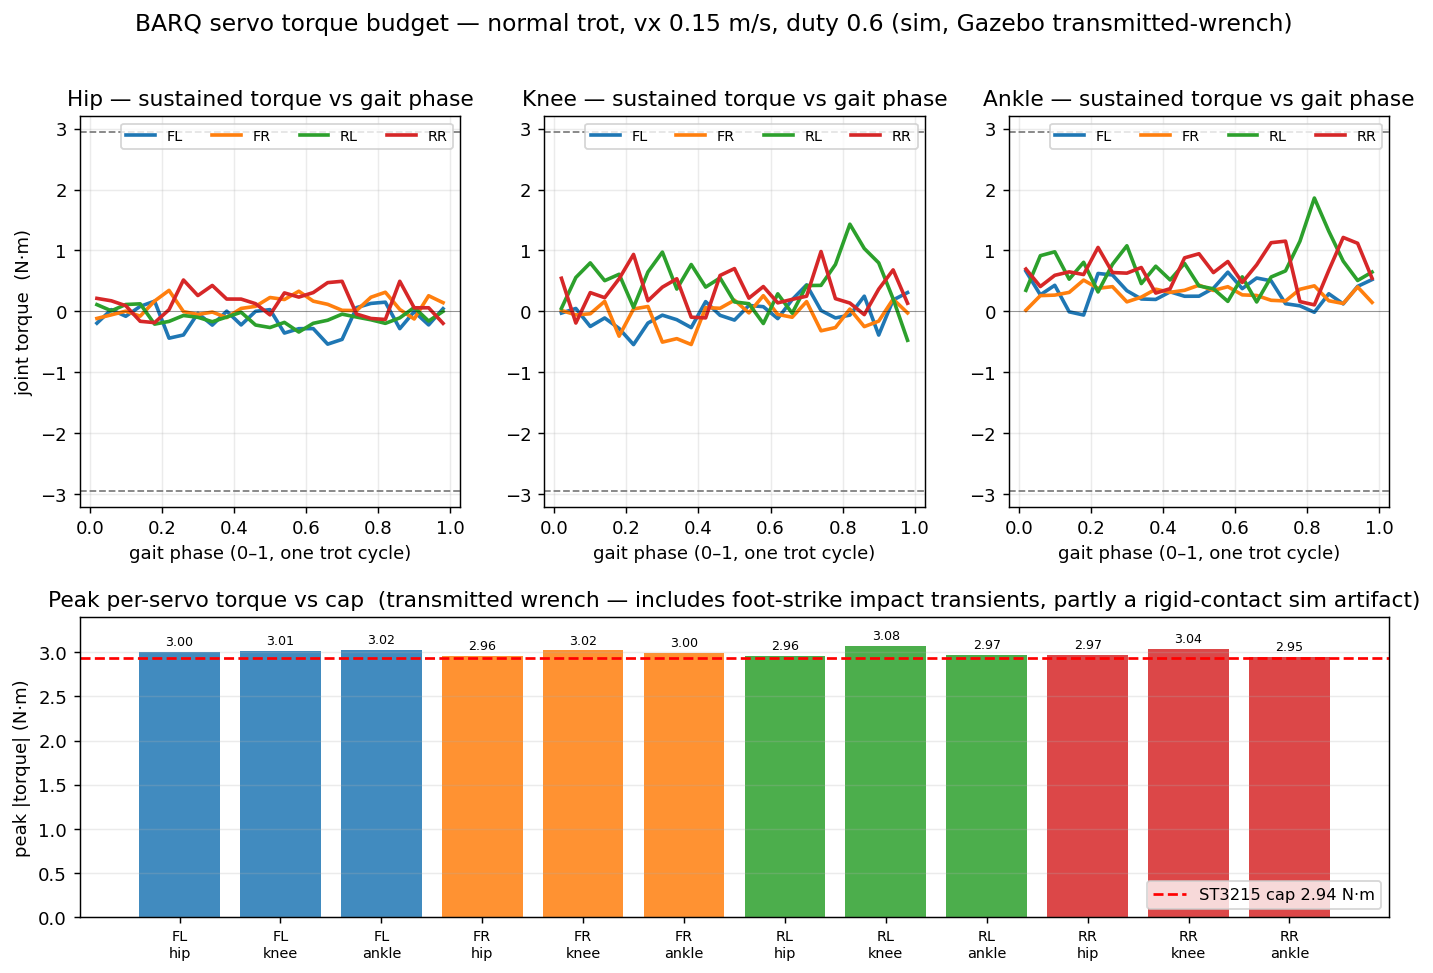
\includegraphics[width=0.92\linewidth]{BARQ_Report_2_fig1.png}
  \caption{Per-servo torque during a normal trot (\textit{vx}~0.15\,m/s). Top: sustained torque
  vs.\ gait phase by joint class. Bottom: peak torque per servo against the 2.94\nm{} actuator cap
  (dashed). Source: simulated joint transmitted-wrench, ground reaction included.}
  \label{fig:torque}
\end{figure}

\section{Quantitative results}
The table below collects the period's primary measured indicators. All figures are reproducible
from the project's versioned tooling and data logs.

\begin{center}\small
\renewcommand{\arraystretch}{1.35}
\begin{tabular}{>{\raggedright\arraybackslash}p{5.6cm} >{\raggedright\arraybackslash}p{3.2cm} >{\raggedright\arraybackslash}p{6.6cm}}
\hline
\textbf{Indicator} & \textbf{Result} & \textbf{Significance}\\
\hline
Model fidelity (settle-height error) & 0.2\,mm & Simulation faithfully matches the modelled machine\\
Joint tracking error (walking) & 17.8\,mrad RMS & Actuator response calibrated to specification\\
Autonomous mission & 16\,m course completed & Final error 0.157\,m; self-recovering\\
Onboard odometry drift & 4--5\% of distance & No external reference required\\
Hardware-interface integration & 9 / 9 checks & Full stack runs without physical hardware\\
Protocol codec tests & 6 / 6 + golden vectors & Computer--microcontroller link verified\\
Control / kinematics test suite & 30 tests passing & Regression-protected\\
Continuous actuator load & 45\% of rated torque & 2.2$\times$ continuous safety margin\\
\hline
\end{tabular}
\end{center}

\section{Engineering process and risk management}
Beyond technical results, the period produced durable process assets that reduce programme risk.
Every engineering decision, change and experiment is recorded in a structured, version-controlled
documentation system, with quantitative before/after metrics retained for eventual publication. The
robot's power architecture has been specified and recorded (a single battery feeding a regulated
motor supply, with a defined low-voltage protection ladder).

Most significantly, a complete execution plan --- spanning calibration, mechanical assembly,
firmware commissioning, first walking, perception, autonomy and machine learning, with measurable
acceptance criteria and explicit contingency procedures at every step --- has been authored as a
self-contained reference. This plan is designed to be executed by a competent engineer without
reliance on any single team member or tool, directly addressing key-person and continuity risk, and
includes a fully specified fallback path to a deployable robot should the most advanced
(machine-learning) approach prove unnecessary or unavailable.

\section{Current status and next steps}
\begin{center}\small
\renewcommand{\arraystretch}{1.35}
\begin{tabular}{>{\raggedright\arraybackslash}p{10.5cm} >{\raggedright\arraybackslash}p{5.9cm}}
\hline
\textbf{Phase} & \textbf{Status}\\
\hline
Simulation, control and inverse kinematics & Complete\\
Physics-fidelity calibration to measured hardware & Complete\\
Perception, SLAM and autonomous navigation & Complete (simulation)\\
Onboard state estimation & Complete (simulation)\\
Embedded protocol and hardware interface & Complete; validated on emulator\\
Physical assembly and commissioning & Ready; awaiting components\\
On-robot walking and autonomy & Planned; fully specified\\
Learned locomotion policy & Planned; three compute paths + fallback\\
\hline
\end{tabular}
\end{center}

\vspace{2mm}
With components now arriving, the immediate next steps are per-servo bench calibration, mechanical
assembly, and firmware commissioning --- each with pre-defined pass/fail gates and contingency
procedures. Because the entire software stack is already proven against an emulated controller, the
transition to physical hardware is expected to be incremental rather than exploratory. We will
report measured on-robot performance against the simulation baselines established in this period in
the next update.

\vspace{6mm}
\begin{center}\itshape --- Aryaman Gupta \& Krish Agarwal\end{center}

\end{document}
